\documentclass[landscape]{article} % kind of document 
\usepackage[utf8]{inputenc} %encoding of choice
\usepackage[american]{babel} %language of choice
\usepackage[p,osf]{cochineal}
\usepackage{fancyhdr} %for header
\usepackage{amsmath, tabu} %math mode
\usepackage{mathtools}
\usepackage{extarrows} % for more options with arrows
\usepackage{amssymb} %math symbols
\usepackage{dsfont} %specifically for the indicator function symbol
\usepackage{xcolor} %to color text
\usepackage{amsthm} %math theorem
\usepackage{tikz}
\usepackage{caption}
\usepackage{multirow}
\usepackage[bottom]{footmisc}
% \usepackage[dvipsnames]{xcolor}
%\usepackage{pythontex}
\usepackage{enumerate} %make lists
\usepackage{graphicx} %insert images
\usepackage{float} %to fix image position
\usepackage{moreverb} %to make boxes
\usepackage{hyperref} %to create hyperlinks
\usepackage{lipsum} %lorem ipsum package
\usepackage{setspace} % to use singlespace below in the solution environment
\usepackage[shortlabels]{enumitem}
\usepackage{parskip}
\usepackage[us]{datetime} %package for setting due date in US format
\newdate{duedate}{6}{12}{2021} %to set a due date
\allowdisplaybreaks
\usepackage[margin=.5in, landscape]{geometry}
\usepackage{rotating}
\usepackage{pdflscape}
\usepackage[paper=portrait,pagesize]{typearea}
\usepackage{jlcode}
\pagestyle{fancy}


\fancypagestyle{mylandscape}{
	\fancyhf{} %Clears the header/footer
	\fancyfoot{% Footer
		\makebox[\textwidth][r]{% Right
			\rlap{\hspace{.75cm}% Push out of margin by \footskip
				\smash{% Remove vertical height
					\raisebox{4.87in}{% Raise vertically
						\rotatebox{90}{\thepage}}}}}}% Rotate counter-clockwise
	\renewcommand{\headrulewidth}{0pt}% No header rule
	\renewcommand{\footrulewidth}{0pt}% No footer rule
}

\lhead{Due: \displaydate{duedate}}
\chead{ECON 899 -- PS3b -- }
\rhead{Danny, Hiroaki, Mitchell, Ryan, Yobin}

\DeclareMathOperator*{\E}{\mathbb{E}} %ease of writing e and E
\newcommand{\e}{\mathrm{e}}
\newcommand{\ct}{\mathsf{c}}
\newcommand{\Z}{\mathbb{Z}}
\newcommand{\R}{\mathbb{R}}
\newcommand{\N}{\mathbb{N}}
\newcommand{\ifn}{\mathds{1}}
\newcommand{\X}{\mathbf{X}}
\newcommand{\Y}{\mathbf{Y}}
\newcommand{\one}{\mathbf{1}}
\newcommand\numberthis{\addtocounter{equation}{1}\tag{\theequation}}
\newcommand*\widebar[1]{\overline{#1}} % to get a widebar
\theoremstyle{definition}
\newtheorem{theorem}{theorem} % Theorem display format
\newtheorem{problem}[theorem]{Exercise} % Problem display format, last bracket sets display choice

\newenvironment{solution}[1][Answer]{\begin{singlespace}\underline{\textbf{#1:}}\quad }{\ \rule{0.3em}{0.3em}\end{singlespace}} % Answer format

\newenvironment{solutions}[1][Proof]{\begin{singlespace}\underline{\textbf{#1:}}\quad }{\ \rule{0.3em}{0.3em}\end{singlespace}} % Answer format
\title{Econ899 PS1b}
\usepackage{listings}

\begin{document}
%\maketitle
The code used to complete this problem set is attached in the appendix below.\footnote{We gratefully acknowledge a conversation with Michael Nattinger that helped us to find an error in applying the Newton method.}
\begin{enumerate}
	\item Problem 1: See inverse\_demand() in functions.jl. The function converges in 73 iterations, and the errors are plotted below.
		\begin{center}
			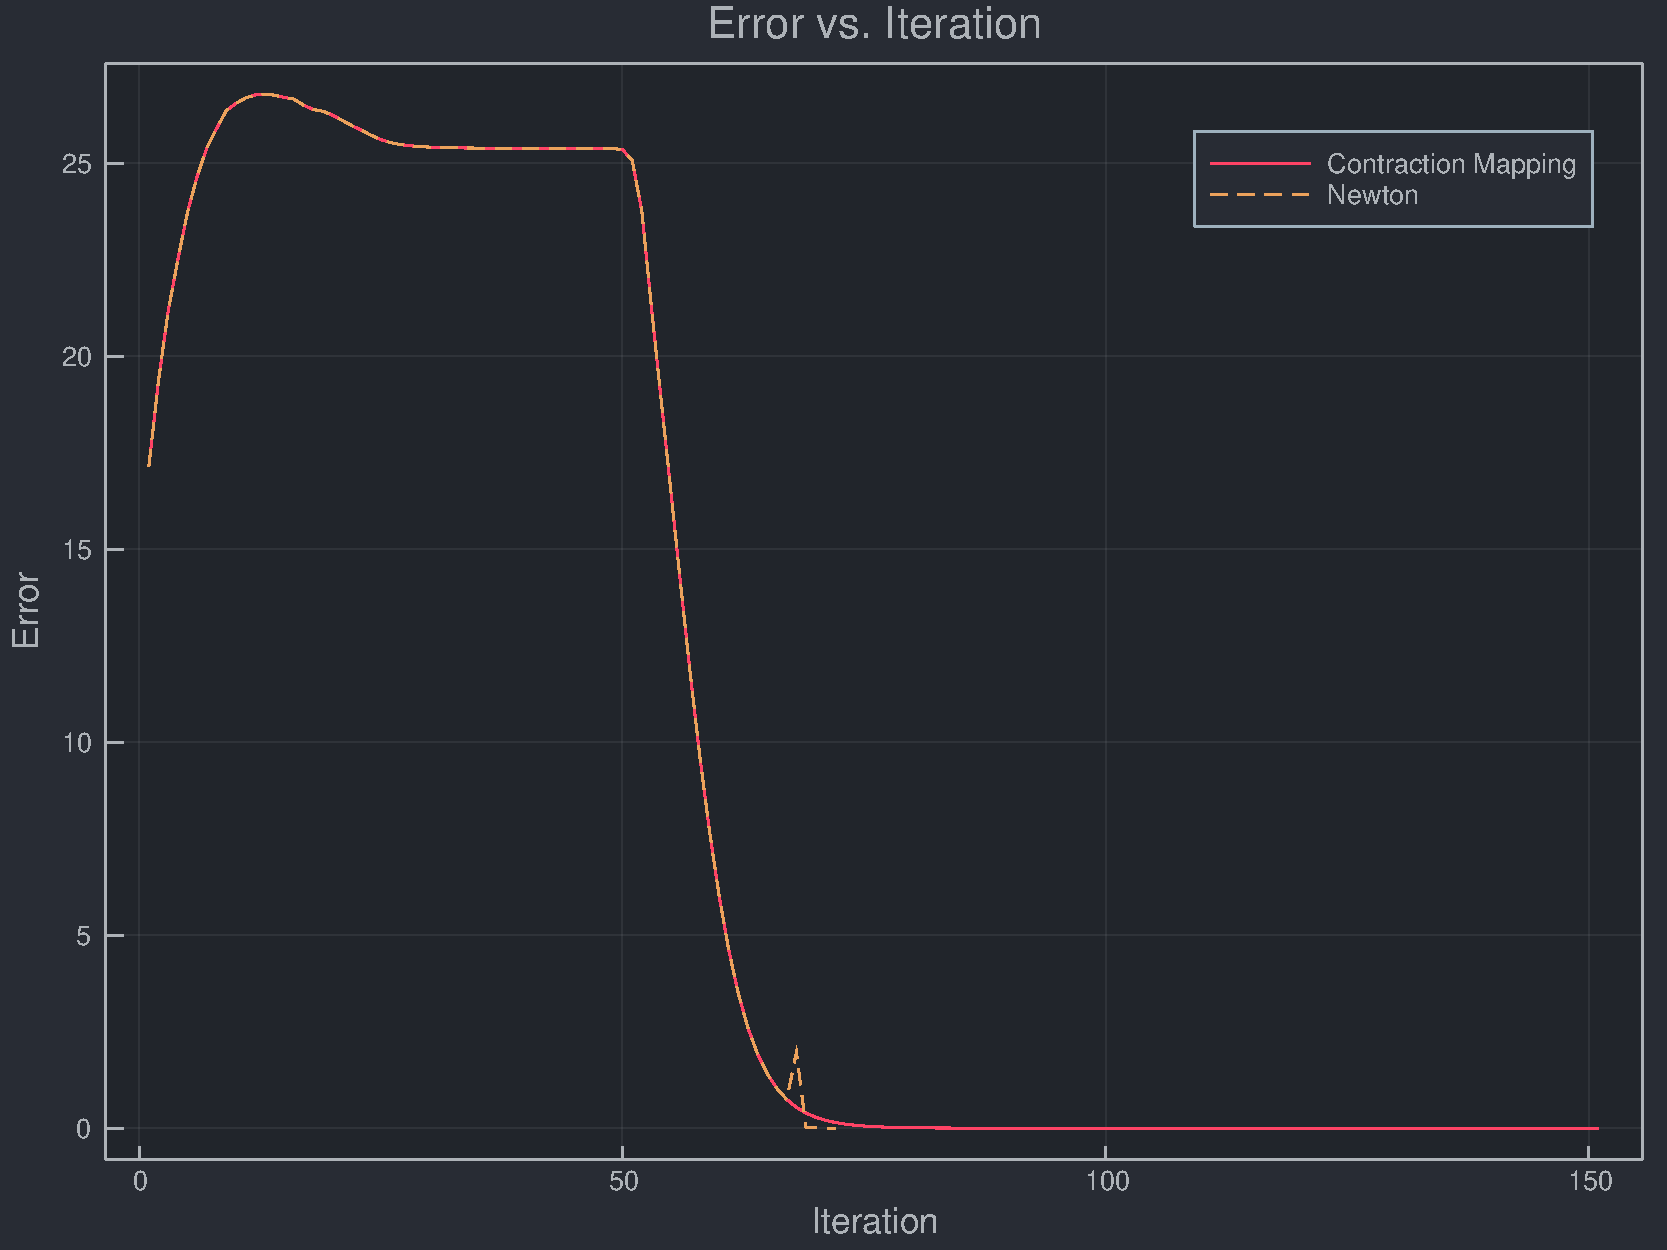
\includegraphics[width=0.8\textwidth]{figures/Problem1.pdf}
		\end{center}

	\item Problem 2: The GMM objective function using the 2SLS weighting matrix is plotted below for $\lambda_p\in[0, 1]$. As you can see, the function is smooth, continuous, and concave with a unique minimum in this range.
		\begin{center}
			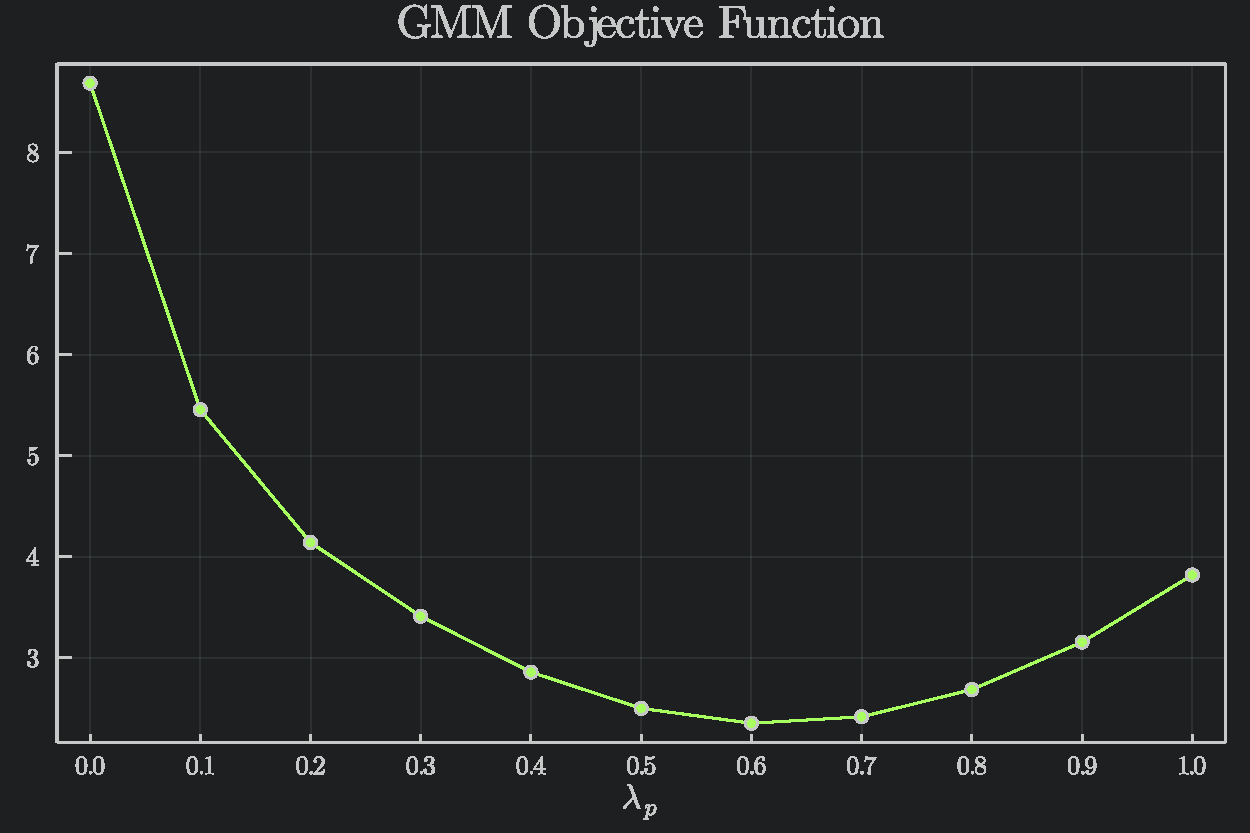
\includegraphics[width=0.8\textwidth]{figures/Problem2.pdf}
		\end{center}

	\item Problem 3: Minimizing the GMM objective function to estimate $\lambda$ with 2-step GMM yields an estimate of $\lambda_p=0.564$.
\end{enumerate}

\newpage
\section*{Appendix}
 	The first codefile named ``runfile.jl" runs the code.
 	\jlinputlisting{Code/runfile.jl}
	
 	The next codefiles, named ``functions.jl," ``manipulate\_data.jl," and ``aux\_vars.jl," are referenced by ``runfile.jl."

 	\jlinputlisting{Code/functions.jl}
	\jlinputlisting{Code/manipulate_data.jl}
	\jlinputlisting{Code/aux_vars.jl}
\end{document}